% Setting up the conference
% Do not edit!
\newif\ifSIGMOD
\SIGMODfalse
\newif\ifVLDB
\VLDBfalse
\newif\ifDRAFT
\DRAFTfalse
\newif\ifARTICLE
\ARTICLEfalse
%%%%%%%%%%%


%%%%%%%%%%%
%Set the type of the document (only one)
%\SIGMODtrue
%\ARTICLEtrue
%\VLDBtrue
%%%%%%%%%%%

%%%%%%%%%%%
%Set whether you want to see the draft version
%\DRAFTfalse %control
%%%%%%%%%%%

% 
\newcommand{\templateName}[0]{}
\newcommand{\varDraft}[0]{}
\ifDRAFT
	\renewcommand{\varDraft}[0]{draft}
\fi
\ifARTICLE
	\renewcommand{\templateName}[0]{article}
\fi
\ifSIGMOD
	\renewcommand{\templateName}[0]{sig-alternate-05-2015}
\fi
\ifVLDB
	\renewcommand{\templateName}[0]{vldb}
\fi

\ifSIGMOD
	\ifARTICLE
		\PackageError{DASlab}{Please use only one document type}{Set only one of the VLDB/SIGMOD/ARTICLE}
		\stop
	\fi
\fi
\ifVLDB
	\ifARTICLE
		\PackageError{DASlab}{Please use only one document type}{Set only one of the VLDB/SIGMOD/ARTICLE}
		\stop
	\fi
\fi
\ifVLDB
	\ifSIGMOD
		\PackageError{DASlab}{Please use only one document type}{Set only one of the VLDB/SIGMOD/ARTICLE}
		\stop
	\fi
\fi


%%%%%%%%%%%
% Setting up the conference
\documentclass[11pt,twocolumn]{article}
\usepackage[margin=1in]{geometry}
\usepackage{setspace}
\setstretch{1}
%%%%%%%%%%%

%%%%%%%%%%%
% WATERMARK
%Fill-in text for side text and watermark
%\newcommand{\sidetext}[0]{\textcopyright 2015 - DASlab - Do Not Distribute}
%\newcommand{\watermark}[0]{DRAFT}
%%\renewcommand{\sidetext}[0]{}
%%\renewcommand{\watermark}[0]{}
%Using above commands to make watermark
%%%%%%%%%%%%%
%Code for the watermark
\usepackage{type1cm,eso-pic}
\makeatletter
\AddToShipoutPicture{%
\setlength{\@tempdimb}{.5\paperwidth}%
\setlength{\@tempdimc}{.5\paperheight}%
\setlength{\unitlength}{1pt}%
\put(\strip@pt\@tempdimb,\strip@pt\@tempdimc){%

\makebox(0,0){\rotatebox{45}{\textcolor[gray]{0.9}%
{\fontsize{3cm}{3cm}\selectfont{ \watermark }}}}%

\makebox(-550,0){\rotatebox{90}{\textcolor[gray]{0.75}%
{\fontsize{0.7cm}{0.7cm}\selectfont{ \sidetext }}}}

}%
}
\makeatother
%%%%%%%%%%
%End of watermark
%%%%%%%%%%%

%%%%%%%%%%%
%Packages, settings and custom commands
%%Standard packages
\usepackage{balance}
\usepackage{color}
%\usepackage{graphicx} %For advances graphics 
%\usepackage{amsmath} %For advanced math symbols
%\usepackage{algorithm2e} %For writing algorithms
%\usepackage{algorithmic} %For the algorithmic environment

%Collaboration
\usepackage{fixme}
%Showing notes only if on draft mode
\ifDRAFT
	\fxsetup{
	    status=draft,
    	author={Note},
	    layout=inline,
    	theme=color,
	    silent=true,
	}
\else
	\fxsetup{
    	status=final,
    	author={Note},
	    layout=pdfnote,
    	theme=color,
	    silent=true,
    	inline=false
	}
\fi

\FXRegisterAuthor{stratos}{astratos}{TODO(si)}
\FXRegisterAuthor{mike}{amike}{\color{blue}{TODO(msk)}}
\FXRegisterAuthor{mark}{amark}{\color{green}{TODO(msk)}}
\newcommand{\si}[1]{\stratoserror{#1}}
\newcommand{\msk}[1]{\mikeerror{#1}}
\newcommand{\mw}[1]{\markerror{#1}}


%Reduce size tools
%Uncommenting pslatex reduces size 
%\usepackage{pslatex}


%Add page numbering if needed
%\pagenumbering{arabic}


%Custom commands
%Boldfaced paragraph
\newcommand{\Paragraph}[1]{\vspace{1.5 mm} \noindent {\bf #1.}}
\newcommand{\ParagraphQ}[1]{\vspace{1.5 mm} \noindent {\bf #1?}}
%Putting figures
\newcommand{\putfigure}[7]
{
\begin{figure}[#1]
\centerline{$
\includegraphics[#2]{#3}
$}
\vspace{#4}
\caption{#5}
\label{#6}
\vspace{#7}
\end{figure}
}



%To signify newly added text
\newcommand{\newtext}[1]{{\color{blue} #1}}
%\renewcommand{\newtext}[1]{#1}



\usepackage{pgfplots}
\usepackage{cite}
\usepackage{hyperref}
%%%%%%%%%%%

\begin{document}
\title{HyperFork: Improving Serverless Latency Through Virtual Machine Flash-Cloning}
  \author{Michael Colavita \hspace{0.5in}
  David Gardner \hspace{0.5in}
  Mark Wilkening}
  \date{Harvard University}

\maketitle

%%%%%%%%%%%
%Examples for figure using custom command:
%\putfigure{1-location}{2-size/options}{3-path}{4-vspace between image and caption}{5-caption}{6-label}{7-vspace below caption}
%\putfigure{t}{width=\columnwidth}{./figures/fig1.pdf}{-0.1in}{This is caption}{fig:label}{-0.1in}
%\putfigure{t}{draft,width=\columnwidth}{./figures/fig1.pdf}{-0.1in}{This is caption}{fig:label}{-0.1in}
%%%%%%%%%%%

\newcommand{\Paragraph}[1]{\vspace{1.5 mm} \noindent {\bf #1.}}
\newcommand{\ParagraphQ}[1]{\vspace{1.5 mm} \noindent {\bf #1?}}

\begin{abstract}
% !TEX root = top.tex
% above command is so that compilation is always from top.tex

Serverless computing provides a convenient infrastructure for performing
computations in response to certain triggers. In most common severless
deployments, computations are executed in virtual machines. As a result, the
boot time of a virtual machine is a primary component of these services'
latency. We propose an alternative paradigm, in which incoming requests trigger
a flash clone of an existing, pre-booted virtual machine. Our implementation
HyperFork builds on top of KVM and utilizes the copy-on-write functionality of
the fork system call to improve performance. We demonstrate that HyperFork
improves virtual machine start times by nearly two orders of magnitude while
maintaining throughput. We find that copy-on-write performance penalties are
minimal for real-world workloads and suggest methods for further improving
throughput.

\end{abstract}

% !TEX root = top.tex above command is so that compilation is always from
% top.tex
\section{Introduction \& Motivation} \label{sec:intro}
\Paragraph{Serverless Computing} Serverless computing, also known as
\emph{Functions-as-a-Service} (FaaS), has become an increasingly important and
desirable platform in the cloud ecosystem. Stemming from the grand vision of
computation as a utility, serverless computing offers users the ability to run
application code directly on a black-box infrastructure. In comparison to
current cloud computing platforms, serverless users (1) no longer have to
manage virtual machine environments, (2) are billed only for application
computation performed in response to requests, and (3) function instances are
auto-scaled to handle dynamically changing request rates. Options are available
from all of the major cloud players, including Amazon Lambda, Azure Functions,
and Google Cloud Functions. Several significant online companies have
implemented parts of their services on serverless platforms, notably the news
site The
Guardian.\footnote{https://aws.amazon.com/solutions/case-studies/the-guardian/}.

\Paragraph{Serverless Infrastructure} The typical implementation of a
serverless computing platform places user-submitted functions onto dynamically
created Virtual Machines (VMs). These functions are intended to be light-weight
stateless single-process programs. Because of the relatively short run-times of
serverless functions, a critical performance constraint in serverless
infrastructure implementations is the scheduling latency of functions -- mainly
comprising of the creation time for instance VMs. A standard optimization
employed for this start-up time is to keep instance VMs running for a period of
time, and schedule function requests onto existing VMs. This leads to a number
of other properties, including limits on function run-time and the potential
for functions to be terminated at any time. This is necessary for the scheduler
to auto-scale instances efficiently. Another property is the clear split in
individual function start-up latencies between \emph{warm-starts}, where a function
is scheduled to an already running instance, and \emph{cold-starts}, where a new VM
must be created for the function. Functions from different users are usually
not placed in the same VM for security and isolation reasons, but one VM can
host several instances of one user's function.

\Paragraph{The Problem with Serverless: Cold-start} A central promise of
serverless computing services is rapid scalability. Meeting this demand at
scale requires that new function instances can be started very quickly to
service incoming requests. This is easy when there exist currently running
warm instances but more difficult when a new cold instance must
be started. A major bottleneck in achieving low latency instance start-up and
fast auto-scaling is the cold-start latency~\cite{peeking}. For cold-start, the
major bottleneck is the creation of a new VM. After scheduling and
provisioning, when a VM is created the host Hypervisor/Virtual Machine Monitor
(VMM) must initialize virtual resources including CPUs, memory, and other
devices, then the guest kernel and file system must be loaded from disk and
initialized in guest memory, then the guest kernel is booted, and finally the
function runtime/process is started and the request is handled.

\Paragraph{Flash Cloning} The most significant parts of VM creation are (1)
copying the kernel and file system into memory, (2) booting the guest kernel,
and (3) loading potentially large libraries/runtimes. Management operations
within the VMM are relatively cheap compared to the start-up within a guest and
the copying of guest memory. Optimizing these steps could dramatically reduce
the startup latency of new serverless functions. One technique to do this is to
employ \emph{flash cloning}. Instead of loading VM images from disk and booting
a kernel, we propose cloning existing reference VMs in memory. Additionally, we
propose a copy-on-write mechanic to reduce both the copy time overhead and the
memory pressure of packing many VMs onto one host. This method can be compared
to the Unix fork abstraction.


\begin{quote} To create an isolated virtual machine, rather than re-create the
entire world, we should only re-create the necessarily distinct VMM components
and clone identical guest memory and execution context from ready-to-go
reference VMs.
\end{quote}

From this insight we present \emph{HyperFork}, a KVM-based VM cloning
implementation for the context of serverless computing.

\Paragraph{Contributions} Our contributions are as follows: \begin{itemize}
\item A KVM based virtual machine cloning implementation which outperforms
standard VM creation latencies by up to AMAZING\%
\item A thorough discussion of the trade-offs related to a number of potential
implementations for VM creation in the context of serverless computing.
\item A thorough analysis of the performance of Hyperfork for both VM creation
latency as well as VM co-location density and performance degredation with
respect to copy-on-write memory sharing.
\end{itemize}

The rest of the paper is organized as follows. Section 2 provides an overview of KVM and the hypervisor \emph{kvmtool}, and then describes the implementation details of \emph{HyperFork}. Section 3 describes our experimental evaluation. Section 4 presents a background and review of related work.

% !TEX root = top.tex
% above command is so that compilation is always from top.tex
\section{Related Work} \label{sec:related}
Our work in this paper draws on concepts from several lines of past research.

% TODO: I'm not convinced the history in this paragraph adds anything to the paper
\Paragraph{Virtualization Technology} Machine virtualization technology is
a complex and diverse space. Classical Hypervisors/Virtual Machine Monitors
(VMMs) relied on the fundamental primitive of \emph{Trap-and-Emulate}, where
sensitive instructions in the guest would be trapped by the hardware, and
emulated safely within the VMM using shadow structures for privileged
state~\cite{classic-virt}. In x86 however, not all sensitive instructions are
privaleged, meaning some cannot be trapped, and other techniques must also be used
to enable virtualization. \emph{Full virtualization} of unmodified guest
kernels was enabled through binary translation, where all sensitive
instructions could be translated into privileged instructions.
\emph{Paravirtualization} used modifications to the guest operating systems to
ensure sensitive operations were trapped. Today, modern hardware architectures
include special virtualization instructions which remove the need for binary
translation, and additionally remove the need for performance critical shadow
structures using two-dimensional hardware page tables~\cite{virt-techniques}.
Current virtualization technologies offer a mix of all these techniques,
including binary translation for full nested virtualization using Oracle's
HVX~\cite{hvx}, paravirtualization with Xen~\cite{xen}, and classic
trap-and-emulate utilizing modern hardware extensions and the QEMU x86
emulator~\cite{qemu} within the Linux kernel with KVM~\cite{kvm}. Xen is highly
used within the research community because of its relatively simple
software-only techniques, and KVM is valued for its tight integration with the
Linux kernel.

% TODO: we need to make the distinction between unikernels and Amazon-style microkernels more clear; we seem to conflate them here
\Paragraph{Cold-start Reduction Efforts} A number of different techniques have
been proposed to reduce cold-start latencies. One broad technique is to reduce
the size and complexity of VMs which are used for serverless functions. Because
serverless functions running in a cloud infrastructure run on a fairly limited
and standard set of physical machines, the number of specialized drivers and
kernel modules required to support this hardware is vastly smaller than that in
a standard distribution.  Additionally, because the function will only need to
run a single process, a number of other optimizations can be made to reduce
kernel size and boot time. Amazon utilizes such a stripped down kernel in their
Firecracker VMM~\cite{firecracker}. These kinds of operating system
optimizations have also been explored previously in a more extreme form, with
Unikernels~\cite{unikernels} and the Denali OS~\cite{denali}, where there is no
real division between operating system and application code.

% TODO: citations
Other approaches to efficient resource isolation put the isolation boundary
above the operating system level. Containerization technologies such as
Docker~\cite{docker} utilize Linux cgroups~\cite{cgroups} and seccomp mechanism
to isolate processes. While these offer very fast startup times compared to
Virtual Machines, they are a weaker form of isolation, as processes in
containers still share a kernel.

Another technique for reducing VM creation latencies involves the process of
\emph{flash-cloning}, in which new VMs are cloned from existing reference VMs.
This is an analogous process to forking processes within linux. One work which
had success with this technique was the Potemkin Virtual
Honeyfarm~\cite{potemkin}. Lightweight VMs were created as Honeypots for
catching security vulnerabilities in cloud applications. This work successfully
implements flash-cloning within the Xen hypervisor~\cite{xen} along with
copy-on-write memory sharing, but focuses on VM density rather than start-up
latency. We implement flash-cloning within a KVM based infrastructure to more
closely match with industry standard serverless infrastructure, Amazon
Firecracker~\cite{firecracker}, and with the goals of minimizing start-up
latency and utilizing native copy-on-write functionality within the Linux
kernel.

\Paragraph{VM Live Migration} Flash-cloning relates very closely to the more
mature virtualization technology of VM live
migration~\cite{post-copy-migration}\cite{snowflock}. Cloud infrastructure has
long required the ability to efficiently migrate VMs across physical hosts. VM
live migration in general contains a superset of the functionality needed for
flash-cloning, but is focused on efficiently supporting the migration of VM
state across a slow network with minimal interruption to the VM. For serverless
computing infrastructure, we are focused on extremely low latency and therefore
do not want the complex techniques used for live-migration. We rely on many
features pioneered by live migration research in order to efficiently duplicate
virtual machine state.

% !TEX root = top.tex
% above command is so that compilation is always from top.tex
\section{Background} \label{sec:background}

In this section we describe the platforms HyperFork is built upon, including an
overview of the KVM hypervisor and kvmtool virtual machine monitor.

\subsection{KVM Overview}

% TODO KVM is ......

A full KVM system contains a number of major components within a Linux host
machine, as depicted in Figure~\ref{fig:kvm-arch}. The KVM kernel module tracks
and maintains most of the sensitive virtualized machine state. Each guest is
isolated within a standard linux process, which contains both VMM management components
as well as the running guest. Within the VMM, management components within the
userspace guest processes communicate with the KVM kernel module via a set of
ioctls. Outside of the guest processes, the VMM contains CLI based management
utility programs for administrators which use IPCs to communicate with the
guest process VMM components. For our implementation, the userspace VMM
components are implemented in kvmtool, however these same fundamental
components will exist in other KVM VMM implementations such as
Firecracker~\cite{firecracker}.

\begin{figure*}[t]
  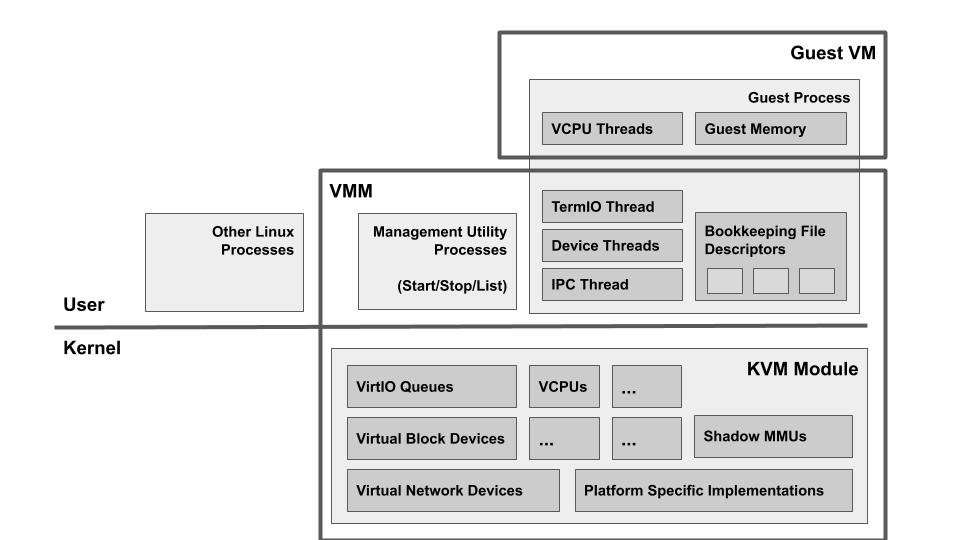
\includegraphics[width=0.8\textwidth]{{figures/kvm-arch}}
  \caption{KVM Software Architecture}
  \label{fig:kvm-arch}
\end{figure*}

\subsection{kvmtool}

kvmtool~\cite{kvmtool} is a VMM implementation for KVM with the minimal
functionality required to boot a fully functional linux kernel with very basic
virtualized devices. Supported devices include block, network, filesystem,
balloon, hardware random number generation, and console virtual devices, along
with a legacy 8250 serial device. kvmtool is provided as an alternative to
heavier VMM solutions such as QEMU~\cite{qemu}, which supports a wide range of
legacy devices and guest configurations.

We selected kvmtool as our userspace VMM as it offers a very similar set of
functionality to Firecracker, the VMM used to power Amazon Lambda. (TODO:
contrast firecracker and kvmtool) We chose kvmtool over Firecracker because we
found that Firecracker was more difficult to work with due to its Rust codebase
and containerization schemes. kvmtool provides a minimal platform on which to
test HyperFork applied to Linux guests and closely approximates the VMM of an
industrial serverless platform.

To virtualize efficiently, kvmtool makes use of a number of threads for
managing vCPUs and emulated devices. Userspace bookkeeping data structures hold
file descriptors which point to the internal VM state maintained within the KVM
kernel module. When the virtual machine is started, kvmtool creates a thread
for each class of device, including the terminal, 8250 serial console, block
devices, and other virtio devices. It then creates several worker threads to
handle arbitrary jobs that may arise from the virtio devices. These tasks
include processing work items from virtio queues and updating the console. In
its default configuration, kvmtool allocates one worker thread for each CPU on
the host machine. As we are virtualizing machines that are much smaller than
the host machine, we limited kvmtool to one worker thread per VM. In addition
to device threads, kvmtool also creates a thread to manage the virtual machines
through IPC calls. This allows administrators to start, pause, stop, and debug
virtual machines using a simple command line interface. Finally, kvmtool
creates one thread per vCPU that proceeds in a loop, invoking the
\texttt{KVM\_RUN} ioctl, then handling any IO requests or interrupts that may
arise. Together, this set of threads enables efficient virtualization of the
guest and its devices.

% !TEX root = top.tex
% above command is so that compilation is always from top.tex

\section{Implementation} \label{sec:implementation}

We now describe the architecture and implementation of Hyperfork, along with
our design decisions regarding the flash-cloning operation.

For a KVM-based virtualization platform, flash-cloning requires duplicating
several pieces of VM state. Where possible, we aim to make heavy use of the
Linux fork operation to duplicate this state, as it is highly optimized and
provides copy-on-write functionality for duplicated pages. Specifically, guest
memory will be shared between the parent and child processes, and will only be
copied if written to. However, the fork system call alone leaves kernelspace
management state unduplicated, cannot duplicate all userspace VMM threads, and
leaves userspace bookkeeping file descriptors pointing to the parent process's
KVM management structures, which are inaccessible in the child.

Duplicating kernel state can either be performed within the kernel, by
coping in-kernel data structures, or in userspace by extracting and saving
guest-specific state in memory before forking. We predict a kernel
implementation may have slightly higher performance, but for simplicity we
implement our flash-cloning entirely in userspace within kvmtool.\footnote{Note
that a kernel implementation would also need to update file descriptors and
their memory mappings. This creates quite a mess in practice.} We also add an
ad-hoc guest-to-host communication channel with an extension to kvmtool to
enable our experimental evaluations.

\subsection{Flash-Cloning Support in kvmtool}

Our userspace HyperFork implementation for kvmtool proceeds in a series of
phases. At a high level, these phases are a triggering event, pre-fork
extraction of kernel state, forking, and post-fork reconstruction of VMM
management state in the child.

First, the fork is triggered, either by an administrator invoking the
\texttt{FORK} IPC via the command line interface, or by the guest sending a
signal to the host indicating that it is ready to fork. In either case, the IPC
thread receives this signal, pauses the virtual machine, and calls the pre-fork
routines.

Because KVM state becomes inaccessible in the child process after the VMM has
forked, all kernel state that must be restored in the child needs to be
recorded by the parent before forking. Alternatively, this could be implemented
by IPC between the parent and child, in which the state is sent after the fork
is complete. We have adopted the former approach. The pre-fork routine thus
saves all individual vCPU state for all vCPUs (registers, interrupt
configuration), global vCPU state (interrupt configuration, clock), and then
locks all mutexes that must survive in the guest. Note that it is not necessary
for the pre-fork routine to save the memory of the virtual machine. As the
memory is mapped in the VMM process, it is unaffected by the fork system call
and remains accessible. It will, however, need to be remapped in the guest
following the fork.

Once the pre-fork routine is complete, kvmtool calls the system call fork. In
the parent, all of the locks acquired by the pre-fork routines are released and
execution proceeds. In the child, the post-fork routine is invoked, performing
the following to reconstruct necessary VMM state:

\begin{enumerate}
\item Acquire new file descriptors for the KVM device and virtual machine
\item Create new file descriptors for the vCPUs
\item Restore individual and global vCPU state\footnote{In the process of
restoring this state, we encountered a bug in how KVM handles setting the
control registers when they change whether the guest is in long mode. We intend
to investigate this further and report it if necessary.}
\item Replace all eventfds used for signaling
\item Create new threads to handle devices and the execution of each vCPU
\item Release all mutexes locked in the pre-fork routine, and replace all
condition variables\footnote{Condition variables must be replaced, as in many
pthread implementations they contain an internal mutex that cannot be locked in
the pre-fork routine. If this mutex is locked by another thread when the IPC
thread performs the fork, the mutex will be permanently locked in the child
process.}
\item Attach the terminal device to a new pseudo-terminal, or detach it to
accept no further input\footnote{Due to a bug in kvmtool, operating with a
pseudoterminal with no slave is not supported.}
\end{enumerate}

Once the post-fork routine is complete, the vCPUs begin executing in the child
and the flash-clone operation is complete.

\subsection{Guest-to-Host Signaling}

For guests with more complex forking behavior, the guest may need to inform the
host when it is ready to fork. For example, a virtual machine running a python
program may chose to fork on boot, after python has started, after modules are
loaded, or after further program initialization has completed. As the guest's
userspace state is very difficult to detect from the VMM, we implement a
rudimentary system for guest-to-host signaling.

The guest-to-host signal consists of sending a message over one of the
processor's ports. This allows for a simple and very efficient way to send
short messages to the host, without requiring any modifications to the guest
kernel. This functionality is accessible from userspace through the C standard
library. We define one message to indicate that the guest is ready to fork, and
one message to indicate that the guest has completed its task. To support our
evaluations, we include in the guest images a \texttt{fork} and \texttt{done}
executable that signal the two events which can be easily executed by guest
benchmarks. Further messages could easily be defined for a more complex
deployment.

% !TEX root = top.tex above command is so that compilation is always from
% top.tex
\section{Evaluation} \label{sec:evaluation} We now describe the
design of our benchmarks for the kvmtool HyperFork implementation. We have
conducted both microbenchmarks, to test the overhead of fork and copy-on-write
page duplication, and end-to-end benchmarks to measure throughput and resource
utilization improvements.

\Paragraph{Experimental Setup}
We perform all tests on an m5.metal instance from Amazon Web Services EC2,
which features 96 logical processors and 384 GB of memory. The file system
image used for all tests is a minimal Linux setup generated using the buildroot
utility.\footnote{buildroot.org} This specially generated image contains only
the minimal set of utilities and software needed for our benchmarks. In typical
use, the guest images used for FaaS platforms may be more fully featured and
optimized, but such single purpose images have no need for the flexibility of a
general purpose Linux distribution image. Since FaaS uses very short-lived
instances, there is no need for package managers, update utilities, or other
maintenance software.

Using a minimal image also presents cold-boot times in an idealistic
environment, as a heavier image would take longer to boot. We therefore show
that our implementation offers substantial start time improvements over even
the best case scenario of cold-booting.

\subsection{Benchmarks}

\Paragraph{Fork Time} As HyperFork replaces the time taken to boot a virtual
machine with the time taken to fork a virtual machine, we run several
experiments to test the time for a VM to fork. These tests start a virtual
machine, run basic userspace initialization, and then fork. The child VMM marks
a timestamp once it finishes restoring KVM state. Figure~\ref{fig:fork-time}
shows the fork time as recorded by the child VM for varying amounts of
allocated guest memory.

As memory is duplicated through copy-on-write in a Linux fork, memory is not
physically copied to the child process unitl it is modified. However, it still
takes time to walk through the parent page table and mark shared memory as
read-only, and generate page tables for the child process. For this reason we
expect to see fork times increase with the amount of memory allocated to the
virtual machine.

We compare the results of this fork time benchmark with the time to cold-boot a
VM.

\Paragraph{Copy-on-Write} Though cloning VMs using fork can decrease
VM start times by orders of magnitude, the guest memory mapped in the parent
and child virtual machine share physical pages until modified. As a result,
modifications to memory in each of the virtual machines can trigger page faults
and memory copies that may degrade performance. We implement a benchmark to
isolate the performance degradation caused by copy-on-write operations after
cloning.

This program begins by allocating some amount of memory, and writes 128 bytes
of random data to each 4096-byte page allocated. This forces pages to be
allocated by the host kernel. It then signals to the host, which forks the VM.
In each child the program then performs an additional pass, again writing
random data to each of those pages.

Each of those post-fork writes will trap into the host kernel and induce a
copy. To assess copy-on-write overhead, we measure the time for each of these
memory passes. We compare passes that trigger a page fault (either due to
allocation pre-fork, or copying post-fork). We also compare passes that do not
trigger a page fault (both pre-fork and post-fork).

\Paragraph{Python Function} In the lifecycle of a typical FaaS request, a VM is
started, any relevant state is loaded, and the user-supplied function is run.
These services mostly use managed runtimes like NodeJS and Python. To simulate
a small latency-sensitive workload, we use the numpy FFT correctness test,
which runs in approximately $2.5$ seconds. This represents a somewhat long
latency sensitive workload, and captures the typical scenario of a function
which starts an interpreter, loads external libraries, and performs a CPU-bound
computation.

We compare the total time of starting 64 separate VMs, and letting each run the
benchmark to completion, with the total time of forking 63 VMs from one
reference image and letting them run to completion. We consider the total CPU
time savings of starting each of these VMs by forking instead of booting. We
also consider a variety of different fork points, including immediately after
boot, after python loads, and after packages are loaded. We also verify that
benchmark performance is not degraded by the forking process.

\subsection{Results}

\begin{figure*}
  \center
  \pgfplotstableread{forktime.tab}{\forktimetable}
  \pgfplotstableread{boottime.tab}{\boottimetable}

  \begin{tikzpicture}
  \begin{axis}[
      width=0.45\textwidth,
      title={Time for Virtual Machine Fork},
      xlabel={Guest Memory (MB)},
      ylabel={Time (ms)},
      xmin=0, xmax=2304,
      ymin=0, ymax=24,
      xtick={0, 512, 1024, 1536, 2048},
      ytick={0, 4, 8, 12, 16, 20, 24},
      ymajorgrids=true,
      xmajorgrids=true,
      grid style=dashed,
  ]

  \addplot+[
      color=blue,
      mark=square,
      only marks,
      error bars/.cd,
      y dir=both, y explicit
      ]
      table [
        y error minus = ly,
        y error plus = hy
      ] {\forktimetable};
  \end{axis}
  \end{tikzpicture}
  \label{fig:fork-time}
  \hspace{1cm}
  \begin{tikzpicture}
  \begin{axis}[
      width=0.45\textwidth,
      title={Time for Virtual Machine Cold Start},
      xlabel={Guest Memory (MB)},
      ylabel={Time (ms)},
      xmin=0, xmax=2304,
      ymin=0, ymax=600,
      xtick={0, 512, 1024, 1536, 2048},
      ytick={0, 100, 200, 300, 400, 500, 600},
      ymajorgrids=true,
      xmajorgrids=true,
      grid style=dashed,
  ]

  \addplot+[
      color=blue,
      mark=square,
      only marks,
      error bars/.cd,
      y dir=both, y explicit
      ]
      table [
        y error minus = ly,
        y error plus = hy
      ] {\boottimetable};
  \end{axis}
  \end{tikzpicture}
  \caption{Time for virtual machine cold start vs. fork}
  \label{fig:boot-time}
\end{figure*}

\Paragraph{Fork Time} Figure~\ref{fig:boot-time} shows our measurement results
for our fork and boot time benchmarks. Error bars indicate the $2.5$- and
$97.5$-percentiles. Using the small image constructed for our benchmarks, we
observed boot times of approximately $563$ ms for a $512$ MB virtual machine.
Boot times increased slightly as memory size increased and overall exhibited
very low variance.

The fork operation, on the other hand, took an average of $7.43$ ms to complete
a fork of a $512$ MB virtual machine. This is an improvement of nearly two
orders of magnitude. Again, we observed very little variance in our
measurements. Fork time appears to scale linearly with the memory size of the
virtual machine, likely because the number of page mappings to be duplicated
scales linearly with the memory size. However, even at large memory sizes,
forking eliminates more than $95$\% of the boot time.

\begin{figure*}

\center

\pgfplotstableread{pagefault.tab}{\cowtable}
\pgfplotstableread{nopagefault.tab}{\memtable}

\begin{tikzpicture}
\begin{axis}[
  width=0.45\textwidth,
  title={Time for Memory Pass, No Page Fault},
	xtick=data,
  symbolic x coords={128,256,512,1024,1536},
	ylabel={Time (ms)},
  xlabel={Pages Touched (MB)},
  legend style={at={(0.05,0.95)},anchor=north west},
	ybar,
	bar width=7pt,
  ymajorgrids=true,
  grid style=dashed
]
\addplot+[
  error bars/.cd,
  y dir=both, y explicit
  ]
  table [
  x = mem,
  y = nofork,
  y error minus = noforklo,
  y error plus = noforkhi
  ] {\memtable};
\addplot+[
  error bars/.cd,
  y dir=both, y explicit
  ]
  table [
  x = mem,
  y = yesfork,
  y error minus = yesforklo,
  y error plus = yesforkhi
  ] {\memtable};
  \legend{Before fork, After fork}
\end{axis}
\end{tikzpicture}
\begin{tikzpicture}
\begin{axis}[
  width=0.45\textwidth,
  title={Time for Memory Pass, With Page Fault},
	xtick=data,
  symbolic x coords={128,256,512,1024,1536},
	ylabel={Time (ms)},
  xlabel={Pages Touched (MB)},
  legend style={at={(0.05,0.95)},anchor=north west},
	ybar,
	bar width=7pt,
  ymajorgrids=true,
  grid style=dashed
]
\addplot+[
  error bars/.cd,
  y dir=both, y explicit
  ]
  table [
  x = mem,
  y = nofork,
  y error minus = noforklo,
  y error plus = noforkhi
  ] {\cowtable};
\addplot+[
  error bars/.cd,
  y dir=both, y explicit
  ]
  table [
  x = mem,
  y = yesfork,
  y error minus = yesforklo,
  y error plus = yesforkhi
  ] {\cowtable};
  \legend{Before fork, After fork}
\end{axis}
\end{tikzpicture}
\caption{Memory benchmark with and without copy-on-write ($n=100$)}
\label{fig:rambench}
\end{figure*}

\Paragraph{Copy-on-Write} Figure~\ref{fig:rambench} shows the results
of our copy-on-write test. Each graph shows the performance before and after
the fork operation. Error bars indicate $2.5$- and $97.5$-percentiles. When
memory writes do not trigger a page fault (left plot), performance does not
appear to change before or after a page fault. This means that after pages have
been allocated (or reallocated after being copied on write), there is no
significant memory performance penalty.

When writes do trigger a page fault (right plot), we observe a considerable
difference before and after the fork operation. Before the fork operation, page
faults occur when we write to pages that have not yet been allocated. The
kernel then allocates a zeroed page and returns. After the fork operation, page
faults trigger a page copy. We observe a roughly $28\%$ performance penalty for
the memory benchmark when pages must be copied. As expected, the benchmark time
scales roughly linearly with the number of pages for which a page fault is
triggered.

\pgfplotstableread[col sep=comma,trim cells=true]{pybench.tab}{\pytable}
\pgfplotstableread[col sep=comma,trim cells=true]{pybenchtimes.tab}{\pytimetable}

\pgfplotsset{compat=1.5}
\begin{figure*}
  \center
  \begin{tikzpicture}[trim axis left, trim axis right]
    \begin{axis}[
        width=0.45\textwidth,
      title={Python Benchmark Cumulative CPU Usage},
      xmin=0,xmax=240,
      ytick=data,
      symbolic y coords={None, After Boot, After Interpreter, After Packages},
      ylabel={Fork Point},
      xlabel={Cumulative CPU Time (s)},
      xbar,
      %bar width=7pt,
      xmajorgrids=true,
      grid style=dashed
    ]
      \addplot+[
        %error bars/.cd,
      %x dir=both, x explicit
    ]
      table [
        y = mode,
      x = total,
      %x error = moe,
    ] {\pytable};
    \end{axis}
  \end{tikzpicture}
  \label{fig:pybench}
\caption{Cumulative CPU time for 64 runs of python benchmark}
\label{fig:pycpu}
\end{figure*}

\begin{figure*}
  \center
  \begin{tabular}{|c|c|c|}
    \hline
    Fork Point & Benchmark Time (ms) & Relative Time \\ \hline
    None & $2500 \pm 9.14$ & $100$\% \\ \hline
    After Boot & $2433 \pm 8.36$ & $97.3$\% \\ \hline
    After Interpreter & $2409 \pm 8.36$ & $96.4$\% \\ \hline
    After Packages & $2401 \pm 8.04$ & $96.0$\% \\ \hline
  \end{tabular}

  \caption{Mean benchmark completion time (with $95$\% confidence interval)}
  \label{fig:pybench}
\end{figure*}


\Paragraph{Python Function} Figure~\ref{fig:pycpu} displays the cumulative CPU
time required for the python benchmark. The margin of error are negligible
(less than $0.2$\%). We see a significant improvement when forking compared to
booting 64 independent virtual machines. Forking after boot immediately results
in a $24.8$\% CPU time savings across the 64 benchmarks. Forking after starting
the python interpreter saves $26.7$\% over not forking. Forking after packages
are loaded saves $30.2\%$ over not forking. Thus forking instead of booting new
virtual machines can result in significant resource savings for servers running
short duration or latency sensitive serverless workloads. This effect would be
accentuated for shorter jobs and more minor for longer ones.

Furthermore, figure~\ref{fig:pybench} shows the mean benchmark completion times
for each forking scheme. Interestingly, we do not observe any performance
degradation when forking instead of booting. In fact, forking exhibits a slight
(but statistically significant) reduction in benchmark completion time. We
suspect this may be due to increased memory locality due to shared pages after
forking.

% !TEX root = top.tex
% above command is so that compilation is always from top.texThis is the conclusions section
\section{Discussion} \label{sec:conclusions}
% TODO: analyze results, hypothesize on causes and solutions, and say how great they are


\section{Conclusion}

We have presented HyperFork, a virtual machine flash-cloning implementation for
serverless computing. Our evaluation demonstrated that HyperFork reduces
virtual machine start time by up to two orders of magnitude while maintaining
end-to-end performance. Furthermore, overall system utilization is drastically
reduced for simultaneous latency-sensitive workloads. Virtual machine cloning
is an effective method for reducing the latency and cost of serverless
deployments.



%%%%%%%%%%%
% you need to run "make fetch-library" in order to copy library in this directory
\bibliographystyle{abbrv}

{
%Uncomment following line to reduce size
%\scriptsize
\bibliography{to-be-added}
}

%%%%%%%%%%%


\end{document}
